\documentclass[12pt, aspectratio=43]{beamer} 

% 自訂字體的封包
\usepackage{fontspec} 

%% 設定中文字體
\usepackage{xeCJK}
    \setCJKmainfont[AutoFakeBold=3]{SimSun}
    \XeTeXlinebreaklocale "zh"             
    \XeTeXlinebreakskip = 0pt plus 1pt

% 數學工具及符號
\usepackage{mathtools, amsmath, amsfonts, amsthm, amssymb, latexsym} 
\usepackage{relsize}
% background
\usetheme{Darmstadt}
\setbeamertemplate{footline}[page number]{}

% Headers and footers
\usepackage{fancyhdr}

% Inserting Images
\usepackage{graphicx}
\usepackage{subcaption}
\usepackage{float}


% Using colours in LaTeX
\usepackage{color}
\usepackage{multirow}

% Biblatex citation styles
\usepackage[style=numeric,backend=bibtex,sorting=none]{biblatex} 
\bibliography{reference}

% Misc
\usepackage{lipsum}
\usepackage{wrapfig}
\usepackage[document]{ragged2e}
\usepackage{tabularx}
\usepackage{tikz}

\usepackage{hyperref}

\setbeamertemplate{caption}[numbered]
 

% Title, Subtitle, Author, Institute, Date
\title[\textbf{TCGA Report}]{TCGA Report}
\author[Chen, Pin-Jui]{Chen, Pin-Jui}
\date[Sep 26, 2025]{Sep 26, 2025}

\begin{document}
	
	% Title page frame
	\begin{frame}
		\titlepage
	\end{frame}
	
	\begin{frame}{Read and Count}
		\begin{figure}[h!]
			\centering
			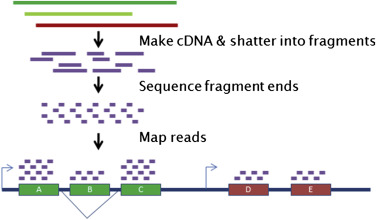
\includegraphics[width=\linewidth]{Read.jpg}
		\end{figure}
	\end{frame}
	
	\begin{frame}{RPKM, FPKM, and TPM}
		RPKM and FPKM formula :
		\begin{center}
			$\dfrac{total \ exon \ reads}{mapped \ reads \ (millions) \ * \ exon \ length (KB)}$
			\end{center}
		TPM formula :
		\begin{center}
			$\dfrac{\dfrac{total \ exon \ reads}{exon \ length(KB)}}{\mathlarger{\sum_{i}}\dfrac{Gene_i \ mapped \ reads (millions)}{exon \ length (KB)}}$
		\end{center}
		In the files GAV2.data and HiSeqV2.data, the data were converted using the $log_2(RPKM + 1)$ transformation.
	\end{frame}
	
	\section{Gene Selection}
	\begin{frame}{Highly Variable Genes (HVG)}
		\begin{enumerate}
			\item \textbf{vst}
			\begin{enumerate}
				\item Fits a line to the relationship of log(variance) and log(mean) using \textbf{loess}.
				\item Standardizes the feature values using the observed mean and expected variance
				\item Clipping to a maximum and calculating feature variance.
			\end{enumerate}
			\item \textbf{mean.var.plot}
			\begin{enumerate}
				\item Calculates $log(\dfrac{variance}{mean})$
				\item Divides features into bins based on their average expression.
				\item Calculates z-scores for dispersion within each bin.
			\end{enumerate}
			\item \textbf{dispersion}
			\begin{enumerate}
				\item Selects the genes with the highest dispersion values.
			\end{enumerate}
		\end{enumerate}
	\end{frame}
	
	\begin{frame}{Differential Expression Analysis (DEA)}
		limma: Linear Models for Microarray Data
	
	\begin{itemize}
		\item \textbf{Purpose:} Identify differentially expressed genes in high-throughput data.
		\item \textbf{Original Use:} Designed for microarray data.
		\item \textbf{Now:} Also applied to RNA-seq data (with voom transformation).
		\item \textbf{Key Ideas:}
		\begin{itemize}
			\item Uses \textbf{linear models} to estimate expression differences.
			\item Applies \textbf{weighted least squares} to account for heteroscedasticity.
			\item Uses \textbf{Empirical Bayes} to stabilize variance estimates and control false positives.
		\end{itemize}
		\item \textbf{Output:} log2 fold change, p-value, and adjusted p-value (FDR).
	\end{itemize}
	
	\end{frame}
	
		
	\begin{frame}{Comparison of Gene Selection Methods}
		
		\begin{block}{Objective}
			Compare three gene selection strategies on PCA and differential expression:
			\begin{itemize}
				\item All genes
				\item Highly Variable Genes (HVG)
				\item Sparse PCA-selected genes
			\end{itemize}
			We perform PCA on HiSeq data, and then fit GA data onto the resulting PCA space.
		\end{block}
		
		\end{frame}
		
		\begin{frame}{Comparison of Gene Selection Methods}
		
		\begin{block}{Workflow}
			\begin{enumerate}
				\item \textbf{Differential Expression Analysis:} 
				\begin{itemize}
					\item Limma on each gene set
					\item Obtain log2 fold-change and adjusted p-values
				\end{itemize}
				
				\item \textbf{Visualization:}
				\begin{itemize}
					\item Volcano plots for each gene set
					\item PCA plots using selected genes
				\end{itemize}
				
				\item \textbf{Overlap Analysis:}
				\begin{itemize}
					\item Count overlapping DE genes between methods
					\item Optional: Venn diagram
				\end{itemize}
			\end{enumerate}
		\end{block}
		
	\end{frame}
	
	
	\begin{frame}{All gene PCA}
		\begin{figure}[h!]
			\centering
			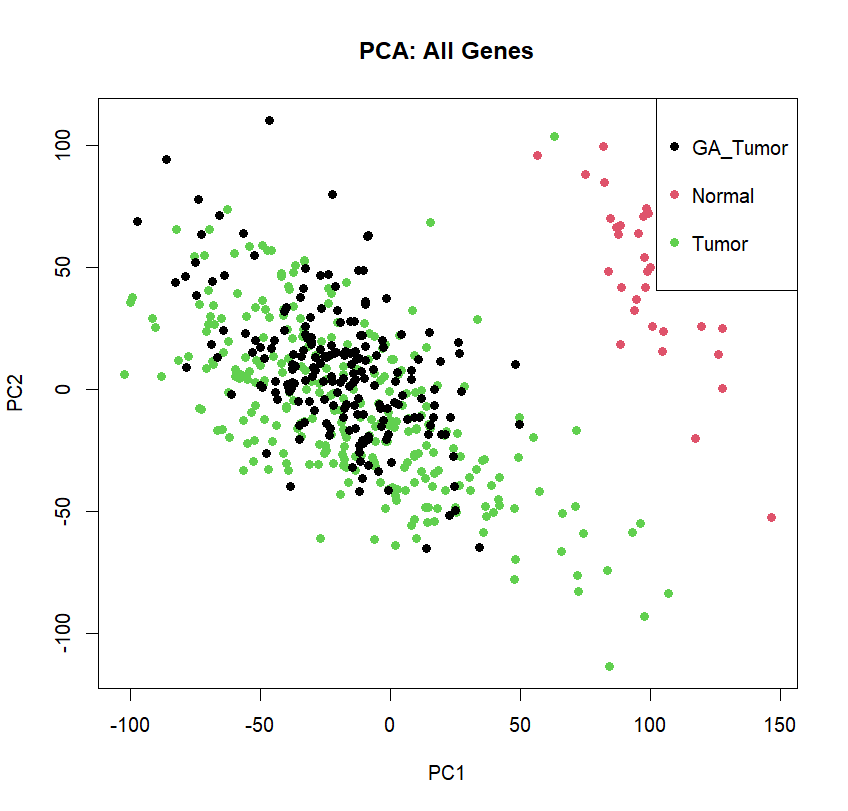
\includegraphics[width=0.8\linewidth]{allgene.png}
		\end{figure}
	\end{frame}
	
	\begin{frame}
		\frametitle{All gene + DEA}
	
			\begin{minipage}[t]{0.50\textwidth} 
				\centering
				\captionof{figure}{DEA Volcano 4806}
				\label{fig:gene-a}
				\vspace{0.5em}
				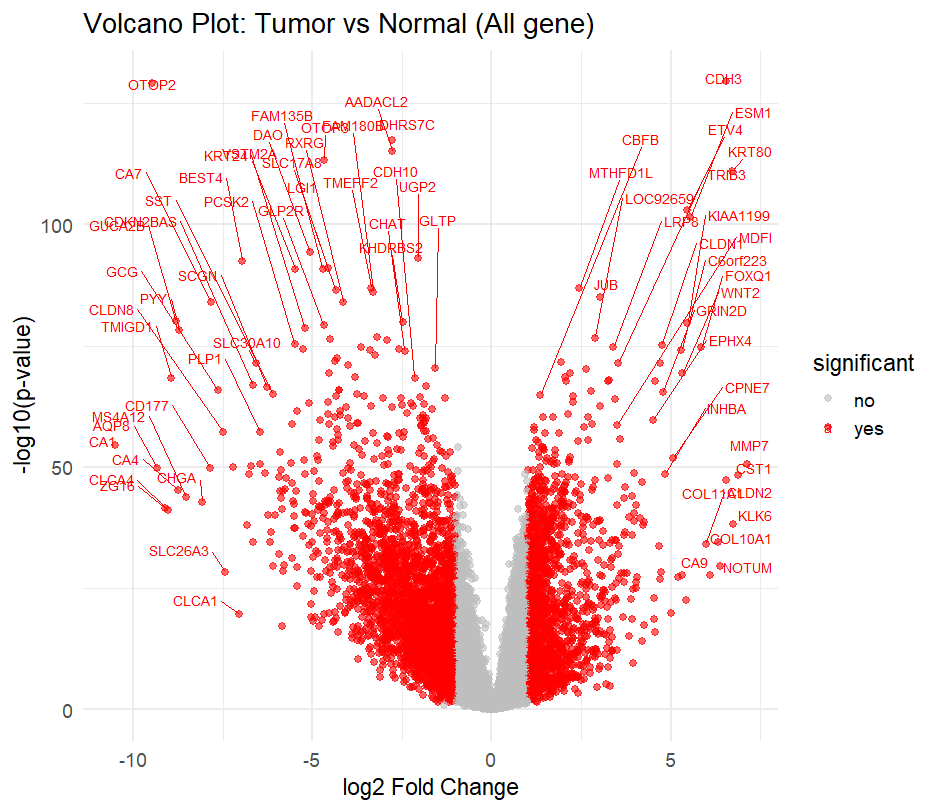
\includegraphics[width=\linewidth]{volcano_dea.png}
	
			\end{minipage}
			\begin{minipage}[t]{0.50\textwidth} 
				\centering
				
				\captionof{figure}{DEA PCA 4806}
				\label{fig:gene-a}
				\vspace{0.5em}
				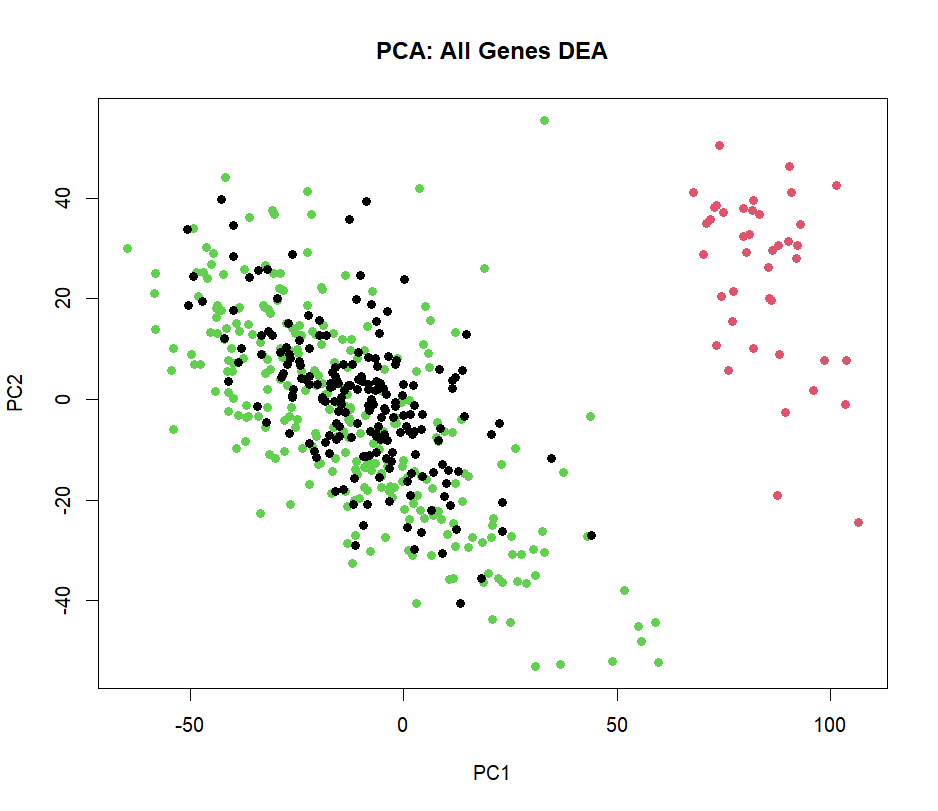
\includegraphics[width=\linewidth]{dea_pca_allgene.png}			
			\end{minipage}%
	
	\end{frame}
	
	\begin{frame}{500 HVG PCA}
		\begin{figure}[h!]
			\centering
			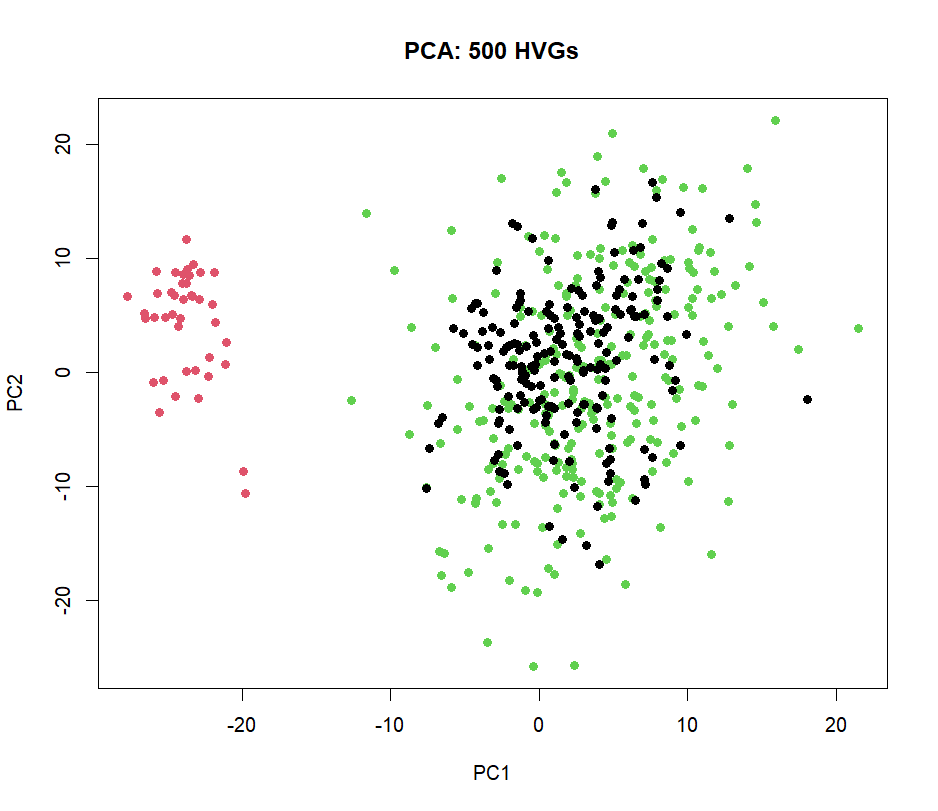
\includegraphics[width=0.8\linewidth]{hvgs.png}
		\end{figure}
	\end{frame}
	
	\begin{frame}
		\frametitle{HVG + DEA}
		
		\begin{minipage}[t]{0.50\textwidth} 
			\centering
			\captionof{figure}{DEA Volcano (369/500)}
			\label{fig:gene-a}
			\vspace{0.5em}
			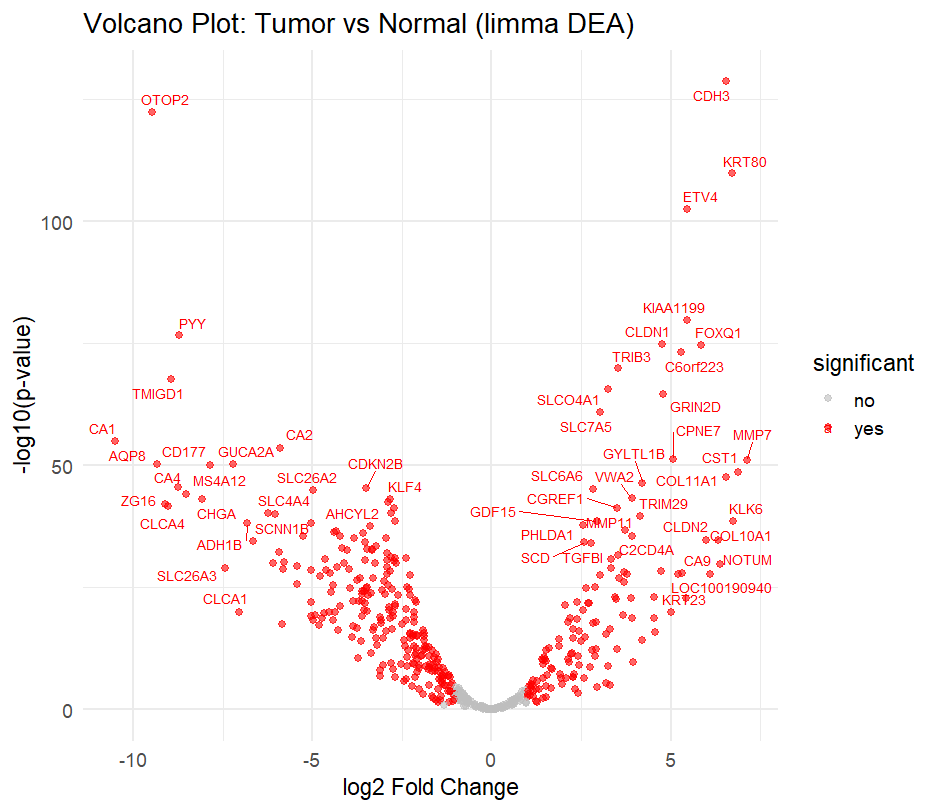
\includegraphics[width=\linewidth]{volcano_hvg.png}
			
		\end{minipage}
		\begin{minipage}[t]{0.50\textwidth} 
			\centering
			
			\captionof{figure}{DEA PCA}
			\label{fig:gene-a}
			\vspace{0.5em}
			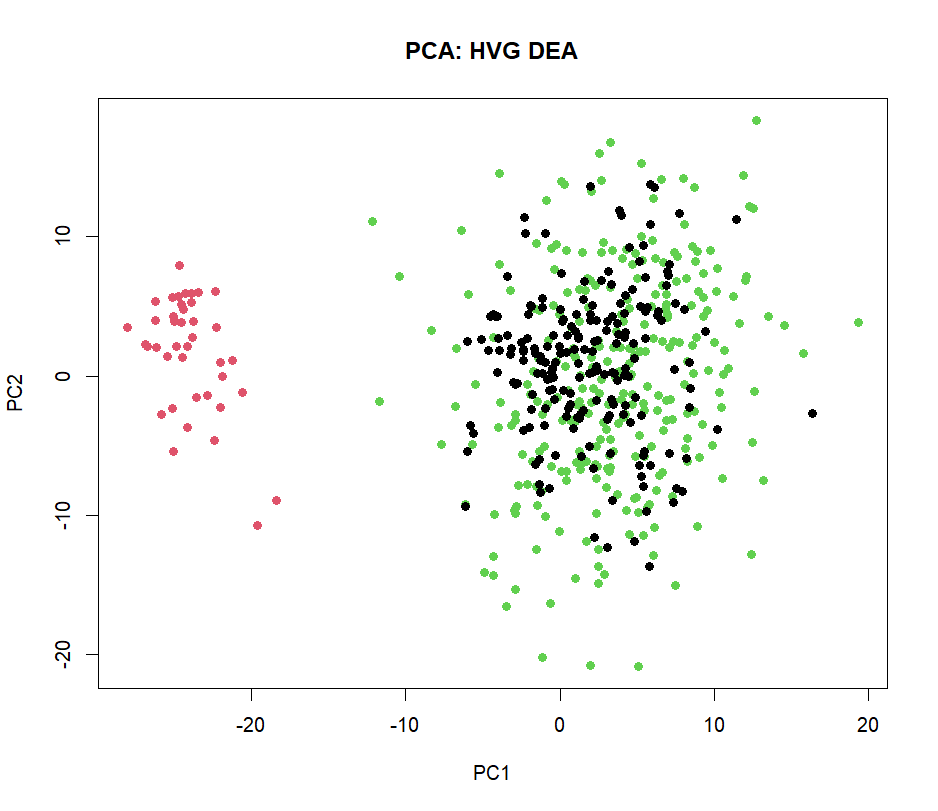
\includegraphics[width=\linewidth]{hvg_dea_pca.png}			
		\end{minipage}%
		
	\end{frame}
	
	
	
	\begin{frame}{Sparse PCA}
		\begin{figure}[h!]
			\centering
			\includegraphics[width=0.8\linewidth]{spca.png}
		\end{figure}
	\end{frame}
	
	\begin{frame}
		\frametitle{SPCA + DEA}
		
		\begin{minipage}[t]{0.50\textwidth} 
			\centering
			\captionof{figure}{DEA Volcano (350/363)}
			\label{fig:gene-a}
			\vspace{0.5em}
			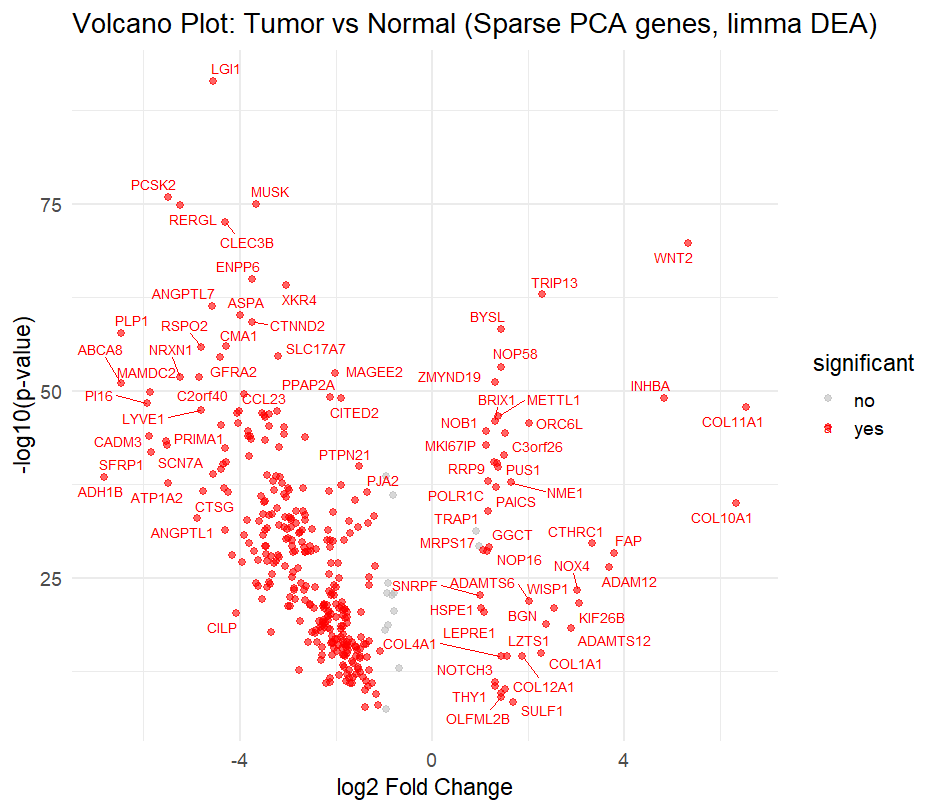
\includegraphics[width=\linewidth]{volcano_spca.png}
			
		\end{minipage}
		\begin{minipage}[t]{0.50\textwidth} 
			\centering
			
			\captionof{figure}{DEA PCA [208,22]}
			\label{fig:gene-a}
			\vspace{0.5em}
			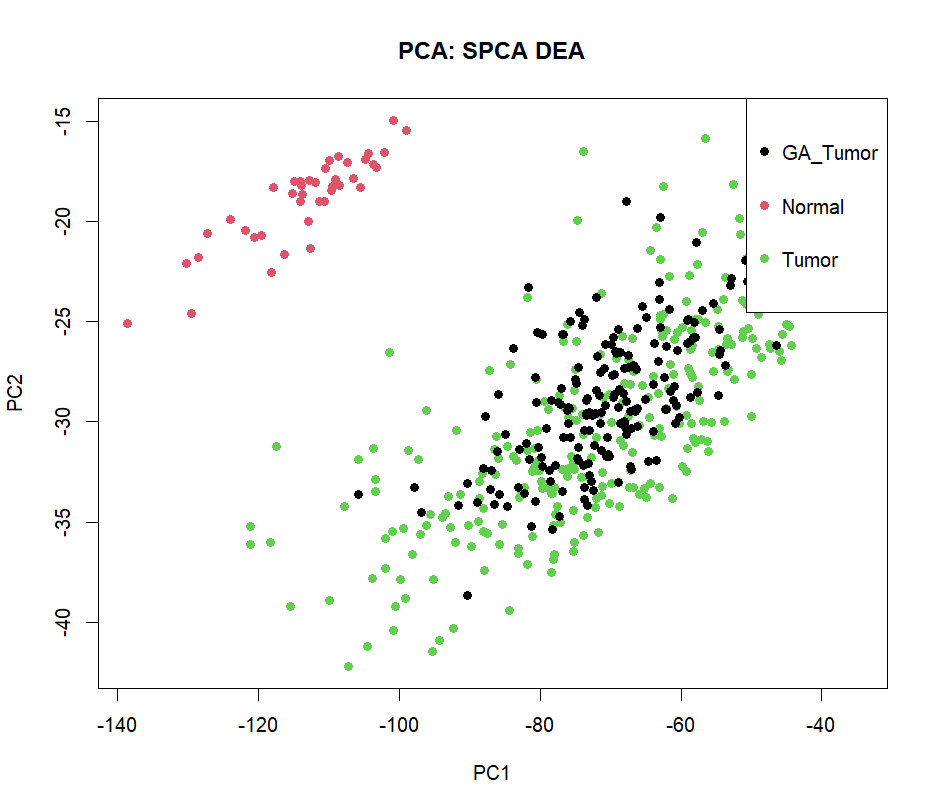
\includegraphics[width=\linewidth]{spca_dea_pca.png}			
		\end{minipage}%
		
	\end{frame}
	
	
	\begin{frame}
		\begin{enumerate}
			\item All gene PCA vs DEA cosine similarity : 
			\\
			PC1 = 0.997 ; PC2 = 0.953
			\item  HVG vs HVG + DEA cosine similarity : 
			\\
			PC1 = -0.977 ; PC2 = 0.919
			\item  SPCA vs SPCA + DEA cosine similarity : 
			\\
			PC1 = -0.944 ; PC2 = 0.924
		\end{enumerate}
	\end{frame}
	
	
	
	\begin{frame}{Intersection DEA, HVG, SPCA}
		\begin{figure}[h!]
			\centering
			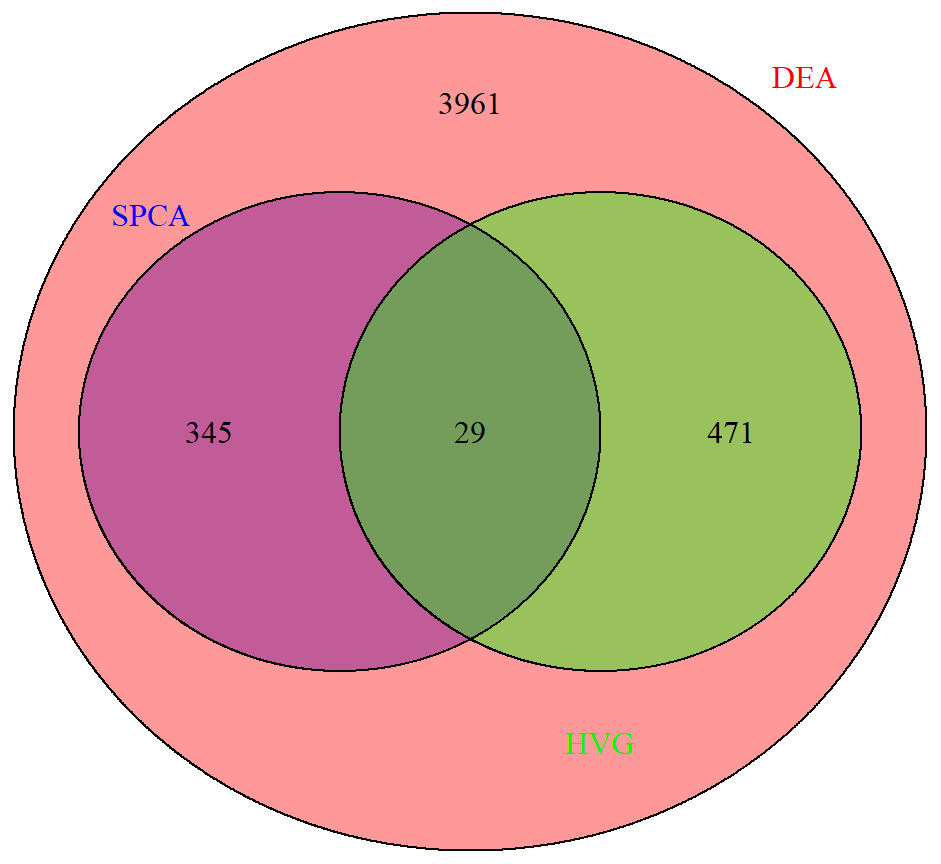
\includegraphics[width=0.8\linewidth]{Venn.png}
		\end{figure}
	\end{frame}
	
	\begin{frame}{HVG + DEA + SPCA}
		\begin{figure}[h!]
			\centering
			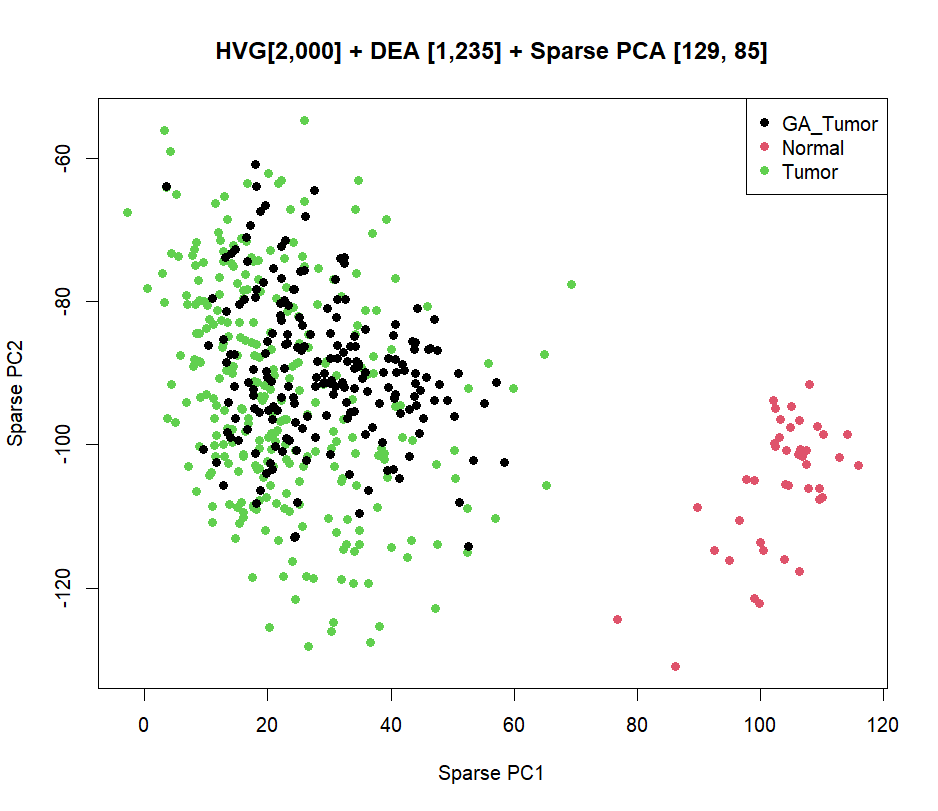
\includegraphics[width=0.8\linewidth]{hvg_dea_spca.png}
		\end{figure}
	\end{frame}
	
\end{document}